%----------------------------------------------------------------------------------------
%	PACKAGES AND OTHER DOCUMENT CONFIGURATIONS
%----------------------------------------------------------------------------------------

\documentclass[11pt,% Default font size
	fleqn,% Left align equations
	a4paper,% Paper size
	twoside% Use two-sided mode instead of oneside
]{backagBook}

% Additional required packages
\usepackage{fontawesome5}% For modern icons
\usepackage{tikz}% For drawing
\usepackage{enumitem}% For description list
\usepackage{needspace}% For better control of page breaks
\usepackage{placeins}% For \FloatBarrier command

% Book information
\hypersetup{pdftitle={Mathématiques - Tronc Commun Scientifique},%
	pdfauthor={Naoufal Labrihmi},%
	pdfsubject={Manuel de Mathématiques pour le Tronc Commun Scientifique - Maroc},%
	pdfkeywords={Mathématiques, Tronc Commun Scientifique, Maroc, Algèbre, Analyse, Exercices, Solutions},%
	pdfcreator={LaTeX},%
        colorlinks=true,% Whether to color links
        %hidelinks,% Hide the default boxes around links
        urlcolor=ocre,% Color for \url and \href links
        linkcolor=black,% Color for \ref/\nameref links
        citecolor=ocre,% Color for reference citations like \cite{}
        hyperindex=true,% Adds links from the page numbers in the index to the relevant page
        linktoc=all% Link from section names and page numbers in the table of contents
}

\addbibresource{sample.bib}

% Define colors based on the provided images
\definecolor{primary}{RGB}{41,67,92}% Deep lake blue
\definecolor{secondary}{RGB}{187,201,215}% Sunset orange
\definecolor{accent1}{RGB}{28,53,56}% Dark teal
\definecolor{accent2}{RGB}{67,108,132}% Misty blue
\definecolor{accent3}{RGB}{12,28,37}% Deep shadow
\definecolor{accent4}{RGB}{187,201,215}% Misty light

% Replace the old ocre color with our primary color
\definecolor{ocre}{RGB}{41,67,92}

\chapterimage{pic2.jpg} % Chapter heading image
\chapterspaceabove{5.8cm} % Default whitespace from the top of the page to the chapter title on chapter pages
\chapterspacebelow{6cm} % Default amount of vertical whitespace from the top margin to the start of the text on chapter pages
\definecolor{partcolor}{RGB}{41,67,92}% Same as primary for part headings

\pdfstringdefDisableCommands{%
  \def\faClipboardCheck{Énoncés}%
  \def\faCalculator{Analyse Réelle}%
  \def\faVectorSquare{Algèbre Linéaire}%
  \def\faLightbulb{Solutions}%
  \def\faTrophy{Olympiades}%
}

\begin{document}

% We don't need this anymore since we've patched the class file
% \let\cleardoublepage\clearpage

\frontmatter
% Title page
\titlepage% Output the title page
    {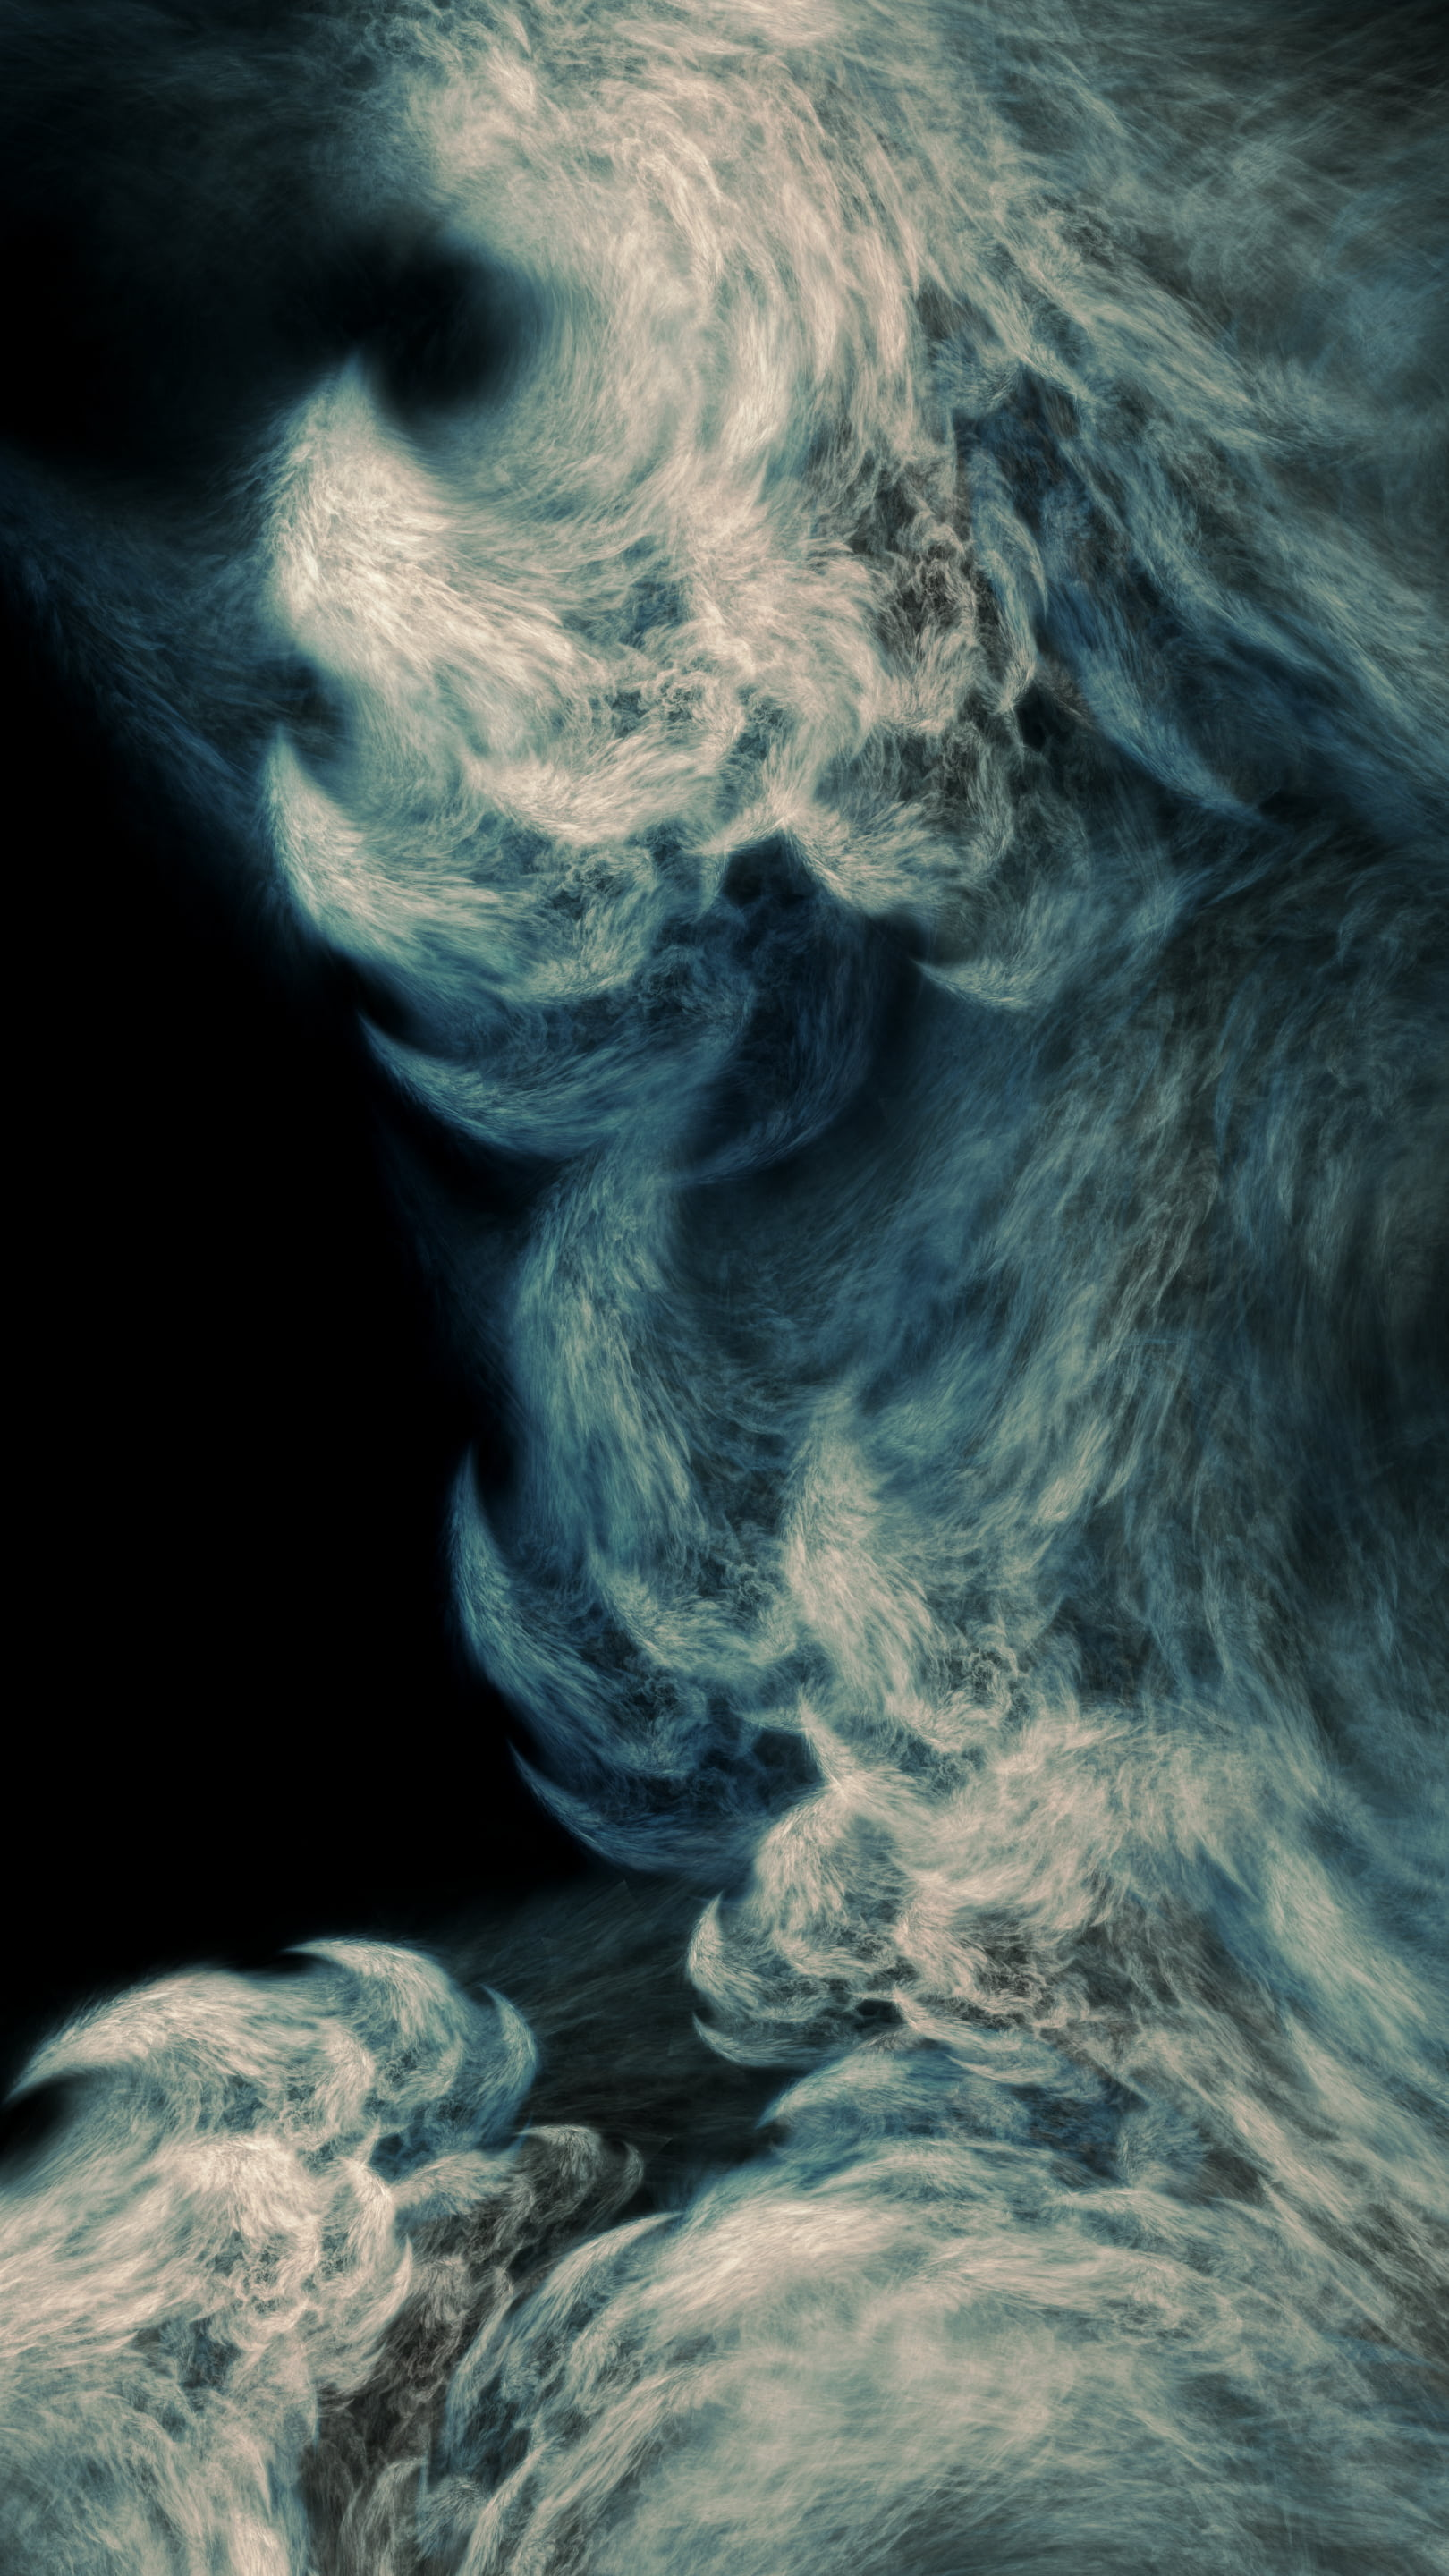
\includegraphics[width=\paperwidth]{Images/peakpx.jpg}}% Background image
    {%
        \centering\sffamily%
        \begin{tikzpicture}[overlay,remember picture]
            % Add semi-transparent overlay to create blur effect
            \fill[black, opacity=0.6] (current page.south west) rectangle (current page.north east);
            
            \node[anchor=north,yshift=-3cm] at (current page.north) {%
                \begin{minipage}{\textwidth}
                    \centering\color{white}%
                    {\fontsize{55}{72}\selectfont\scshape\bfseries\hspace*{0pt}\mbox{MATHÉMATIQUES}\par}%
                    \vspace{1cm}%
                    {\LARGE\scshape Tronc Commun Scientifique\par}%
                    \vspace{0.5cm}%
                    {\Large\itshape De la Théorie à l'Excellence\par}%
                \end{minipage}
            };
            
            \node[anchor=center,yshift=0cm] at (current page.center) {%
                \begin{minipage}{\textwidth}
                    \centering
                    \begin{tabular}{@{}c@{\hspace{3cm}}c@{}}
                        \multicolumn{2}{c}{\color{secondary}\Huge\faBookOpen}\\[0.3cm]
                        \multicolumn{2}{c}{\color{white}\Large\scshape Cours Complets}\\[1.5cm]
                        {\color{secondary}\Huge\faEdit} & {\color{secondary}\Huge\faTasks}\\[0.3cm]
                        {\color{white}\Large\scshape Exercices Résolus} & {\color{white}\Large\scshape Devoirs avec Solutions}\\[1.5cm]
                        \multicolumn{2}{c}{\color{secondary}\Huge\faTrophy}\\[0.3cm]
                        \multicolumn{2}{c}{\color{white}\Large\scshape Problèmes d'Olympiade}
                    \end{tabular}
                \end{minipage}
            };
            
            \node[anchor=south,yshift=3cm] at (current page.south) {%
                \begin{minipage}{\textwidth}
                    \centering\color{white}%
                    {\Large\bfseries Pr. SARDI OTHMANE\par}%
                    \vspace{0.4cm}%
                    {\large\scshape Professeur de Mathématiques\par}%
                    \vspace{0.4cm}%
                    {\large\scshape Crmef Safi\par}%
                \end{minipage}
            };
        \end{tikzpicture}
    }

% Copyright page


\thispagestyle{empty}

~\vfill % Push the text down to the bottom of the page

\noindent Copyright \copyright\ 2025 Naoufal Labrihmi\\ % Copyright notice
\noindent \textsc{Published by Naoufal Labrihmi}\\ % Publisher
\noindent \textsc{\href{https://github.com/NaoufalLabrihmi}{github.com/NaoufalLabrihmi}}\\ % URL
\noindent Licensed under the MIT License. Permission is hereby granted, free of charge, to any person obtaining a copy of this software and associated documentation files, to deal in the Software without restriction, including without limitation the rights to use, copy, modify, merge, publish, distribute, sublicense, and/or sell copies of the Software.\\ % License information
\noindent \textit{First printing, \today} % Printing/edition date

%----------------------------------------------------------------------------------------
%	REMERCIEMENTS
%----------------------------------------------------------------------------------------

\clearpage % Replace \cleardoublepage with \clearpage
\thispagestyle{empty}

\begin{center}
    \vspace*{2cm}
    {\LARGE\bfseries\sffamily\color{primary}Remerciements}\par
    \vspace{1.5cm}
\end{center}

\vspace{0.5cm}

Je tiens à exprimer ma sincère gratitude au Professeur SARDI OTHMANE pour son encadrement exceptionnel, son soutien constant et ses précieux conseils tout au long de l'élaboration de ce projet.

\vspace{0.5cm}

Ce travail a été réalisé dans le cadre du programme de formation au Centre Régional des Métiers de l'Éducation et de la Formation (CRMEF) de Safi, promotion 2024-2025.

\vspace{0.5cm}

Je remercie également tous mes collègues de promotion pour les discussions enrichissantes et l'atmosphère collaborative qui ont grandement contribué à la qualité de ce document.

\vspace{0.5cm}

Ce manuel est dédié aux élèves du Tronc Commun Scientifique au Maroc, avec l'espoir qu'il puisse faciliter leur apprentissage des mathématiques et les inspirer à poursuivre leur exploration dans ce domaine fascinant.

%----------------------------------------------------------------------------------------
%	À PROPOS
%----------------------------------------------------------------------------------------

\clearpage % Replace \cleardoublepage with \clearpage
\thispagestyle{empty}

\begin{center}
    \vspace*{2cm}
    {\LARGE\bfseries\sffamily\color{primary}À Propos de ce Document}\par
    \vspace{1.5cm}
\end{center}

\textbf{Contexte et objectif}

\vspace{0.3cm}
Ce manuel de mathématiques a été conçu spécifiquement pour les élèves du Tronc Commun Scientifique au Maroc. Il s'inscrit dans le cadre d'un projet pédagogique réalisé au CRMEF de Safi sous la supervision du Professeur SARDI OTHMANE.

\vspace{0.5cm}

\textbf{Structure du document}

\vspace{0.3cm}

Le manuel est organisé en plusieurs parties :
\begin{itemize}
    \item \textbf{Cours théoriques} : Présentations claires et structurées des concepts mathématiques fondamentaux.
    \item \textbf{Exercices avec solutions} : Problèmes résolus illustrant l'application des théories.
    \item \textbf{Devoirs} : Séries d'exercices progressifs pour approfondir la compréhension.
    \item \textbf{Solutions détaillées} : Explications pas à pas pour favoriser l'apprentissage autonome.
    \item \textbf{Problèmes d'Olympiade} : Défis mathématiques pour stimuler la réflexion avancée.
\end{itemize}

\vspace{0.5cm}

\textbf{Approche pédagogique}

\vspace{0.3cm}
Ce document adopte une approche progressive, partant des concepts fondamentaux vers des applications plus complexes. Chaque notion est illustrée par des exemples concrets et suivie d'exercices de difficulté croissante, permettant aux élèves de consolider leurs acquis étape par étape.

\vspace{0.5cm}

\textbf{Public cible}

\vspace{0.3cm}

Bien que principalement destiné aux élèves du Tronc Commun Scientifique au Maroc, ce manuel peut également servir de ressource complémentaire pour les enseignants et les élèves des premières années universitaires.

%----------------------------------------------------------------------------------------
%	TABLE OF CONTENTS
%----------------------------------------------------------------------------------------

\pagestyle{empty} % Disable headers and footers for the following pages

\tableofcontents % Output the table of contents

\pagestyle{fancy} % Enable default headers and footers again

\clearpage % Start the following content on a new page

\mainmatter


%----------------------------------------------------------------------------------------
%	PREMIER SEMESTRE
%----------------------------------------------------------------------------------------

\part{Premier Semestre}
\chapterimage{pic1.jpg}
\chapter{Analyse Réelle}

\section{Concepts Fondamentaux}

\begin{definition}[Limite d'une fonction]
Soit $f: D \to \mathbb{R}$ une fonction et $a$ un point d'accumulation de $D$. On dit que $L$ est la limite de $f$ en $a$ si:
\[\forall \varepsilon > 0, \exists \delta > 0, \forall x \in D, 0 < |x-a| < \delta \Rightarrow |f(x)-L| < \varepsilon\]
\end{definition}

\begin{notation}[Notation de limite]
On note:
\[\lim_{x \to a} f(x) = L\]
pour indiquer que $L$ est la limite de $f$ en $a$.
\end{notation}

\begin{theorem}[Unicité de la limite]
Si une fonction admet une limite en un point, cette limite est unique.
\end{theorem}

\begin{proof}
Supposons que $f$ admette deux limites $L_1$ et $L_2$ en $a$.
Soit $\varepsilon > 0$. Il existe $\delta_1, \delta_2 > 0$ tels que:
\begin{align*}
|x-a| < \delta_1 &\Rightarrow |f(x)-L_1| < \frac{\varepsilon}{2} \\
|x-a| < \delta_2 &\Rightarrow |f(x)-L_2| < \frac{\varepsilon}{2}
\end{align*}
Donc pour $|x-a| < \min(\delta_1,\delta_2)$:
\[|L_1-L_2| \leq |f(x)-L_1| + |f(x)-L_2| < \varepsilon\]
Comme ceci est vrai pour tout $\varepsilon > 0$, on a $L_1 = L_2$.
\end{proof}

\begin{proposition}[Opérations sur les limites]
Si $\lim_{x \to a} f(x) = L$ et $\lim_{x \to a} g(x) = M$, alors:
\begin{enumerate}
    \item $\lim_{x \to a} (f+g)(x) = L + M$
    \item $\lim_{x \to a} (fg)(x) = LM$
    \item Si $M \neq 0$, $\lim_{x \to a} \frac{f}{g}(x) = \frac{L}{M}$
\end{enumerate}
\end{proposition}

\begin{example}[Calcul de limite]
Calculons $\lim_{x \to 0} \frac{\sin x}{x}$.
\begin{enumerate}
    \item Cette forme est indéterminée (0/0)
    \item On peut utiliser l'inégalité $|\sin x| \leq |x|$
    \item Et le fait que $\cos x \to 1$ quand $x \to 0$
    \item Donc $\lim_{x \to 0} \frac{\sin x}{x} = 1$
\end{enumerate}
\end{example}

\begin{corollary}[Continuité des fonctions rationnelles]
Toute fonction rationnelle est continue sur son domaine de définition.
\end{corollary}

\begin{remark}[Importance des hypothèses]
Dans le théorème d'unicité de la limite, l'hypothèse que $a$ est un point d'accumulation est essentielle. Sans cette hypothèse, une fonction pourrait avoir plusieurs limites ou aucune limite.
\end{remark}

\begin{vocabulary}[Point d'accumulation]
Un point $a$ est un point d'accumulation d'un ensemble $E$ si tout voisinage de $a$ contient une infinité de points de $E$ différents de $a$.
\end{vocabulary}

\begin{problem}[Limite et continuité]
Soit $f: \mathbb{R} \to \mathbb{R}$ une fonction continue sur $\mathbb{R}$ telle que $\lim_{x \to +\infty} f(x) = \lim_{x \to -\infty} f(x)$. Montrer que $f$ admet un minimum ou un maximum global.
\end{problem}

\section{Exercices avec Solutions}\label{sec:exercices-solutions}

\begin{exercise}
Montrer que $\sqrt{2}$ est irrationnel.
\end{exercise}

\begin{solution}
Démonstration par l'absurde:
\begin{enumerate}
    \item Supposons que $\sqrt{2}$ est rationnel
    \item Alors $\sqrt{2} = \frac{p}{q}$ avec $p,q$ entiers premiers entre eux
    \item Donc $2q^2 = p^2$
    \item Donc $p^2$ est pair, donc $p$ est pair
    \item Posons $p = 2k$, alors $2q^2 = 4k^2$
    \item Donc $q^2 = 2k^2$
    \item Donc $q$ est pair
    \item Contradiction car $p$ et $q$ sont premiers entre eux
\end{enumerate}
\end{solution}

\begin{exercise}
Démontrer que pour tout $x \in \mathbb{R}$, on a $|x| \leq 1 + x^2$.
\end{exercise}

\section{Exercices d'Entraînement}\label{sec:exercices-entrainement}

\begin{exercise}
Soit $E$ un sous-ensemble non vide et majoré de $\mathbb{R}$. Montrer que $\sup(E+1) = \sup(E) + 1$.
\end{exercise}

%----------------------------------------------------------------------------------------
%	EXAMPLE CHAPTERS (KEEPING AS REQUESTED)
%----------------------------------------------------------------------------------------

\chapter{In-text Element Examples}
tesing testing testing
\section{Remarks}\index{Remarks}

This is an example of a remark.

\begin{remark}
    The concepts presented here are now in conventional employment in mathematics. Vector spaces are taken over the field $\mathbb{K}=\mathbb{R}$, however, established properties are easily extended to $\mathbb{K}=\mathbb{C}$.
\end{remark}

%----------------------------------------------------------------------------------------
%	DEUXIÈME SEMESTRE
%----------------------------------------------------------------------------------------

\part{Deuxième Semestre}
\chapter{Algèbre Linéaire}

\section{Espaces Vectoriels}

\begin{definition}[Espace vectoriel]
Un espace vectoriel sur un corps $\mathbb{K}$ est un ensemble $E$ muni d'une addition et d'une multiplication externe satisfaisant les axiomes usuels.
\end{definition}

\begin{theorem}[Dimension d'un espace vectoriel]
Deux bases d'un même espace vectoriel ont le même cardinal.
\end{theorem}

\begin{remark}[Référence bibliographique]
Pour plus d'informations sur ce sujet, voir \cite{Smith:2021qr} et \cite{Naoufal:2025jd}.
\end{remark}

\section{Exercices avec Solutions}

\begin{exercise}
Soit $E$ un espace vectoriel de dimension finie. Montrer que toute famille de vecteurs dont le cardinal est strictement supérieur à la dimension de $E$ est liée.
\end{exercise}

\begin{solution}
Soit $n = \dim E$ et $(v_1, \ldots, v_{n+1})$ une famille de $n+1$ vecteurs.
\begin{enumerate}
    \item Soit $(e_1, \ldots, e_n)$ une base de $E$
    \item Pour tout $i$, $v_i$ s'écrit comme combinaison linéaire des $e_j$
    \item Le système d'équations obtenu a plus d'inconnues que d'équations
    \item Donc il admet une solution non triviale
    \item Cette solution donne une relation de liaison entre les $v_i$
\end{enumerate}
\end{solution}

\section{Exercices d'Entraînement}

\begin{exercise}
Soit $E$ un espace vectoriel et $F$ un sous-espace de $E$. Montrer que si $\dim F = \dim E$, alors $F = E$.
\end{exercise}

%----------------------------------------------------------------------------------------
%	DEVOIRS
%----------------------------------------------------------------------------------------

\part{Devoirs}
\chapterimage{pic2.jpg} % Use a different chapter image for assignments
\chapterspaceabove{6cm}
\chapter{{\faClipboardCheck} Énoncés des Devoirs}

\section{\protect\faCalculator\ Analyse Réelle}

\subsection{Devoir 1}

\subsubsection{Type A}
\begin{exercise}
Étudier la convergence de la suite définie par:
\[u_n = \left(1 + \frac{1}{n}\right)^n\]
\end{exercise}

\begin{exercise}
Déterminer les valeurs de $a$ pour lesquelles la série $\sum_{n=1}^{\infty} \frac{n^a}{2^n}$ converge.
\end{exercise}

\subsubsection{Type B}
\begin{exercise}
Soit $f:\mathbb{R} \to \mathbb{R}$ définie par $f(x) = e^x - x - 1$. Montrer que $f(x) > 0$ pour tout $x \neq 0$.
\end{exercise}

\begin{exercise}
Étudier la convergence de la série $\sum_{n=1}^{\infty} \frac{n!}{n^n}$.
\end{exercise}

\section{\protect\faVectorSquare\ Algèbre Linéaire}

\subsection{Devoir 2}
\subsubsection{Type C}
\begin{exercise}
Soit $A$ une matrice carrée d'ordre $n$. On note $\chi_A(X)$ son polynôme caractéristique. Montrer que $\chi_A(A) = 0$.
\end{exercise}

\begin{exercise}
Déterminer les valeurs propres et les vecteurs propres de la matrice:
\[
A = \begin{pmatrix}
3 & 1 & 1 \\
1 & 3 & 1 \\
1 & 1 & 3
\end{pmatrix}
\]
\end{exercise}

\chapterimage{pic2.jpg} % Use a different chapter image for solutions
\chapterspaceabove{6cm}
\chapter{{\faLightbulb} Solutions des Devoirs}

\section{\protect\faCalculator\ Analyse Réelle}

\subsection{Devoir 1}
\subsubsection{Type A}

\begin{solution}
\textbf{Solution de l'Exercice 1:}
\begin{enumerate}
    \item On montre d'abord que la suite $(u_n)$ est croissante
    \item Puis on montre qu'elle est majorée
    \item On utilise le développement en série:
          \begin{align*}
          \left(1 + \frac{1}{n}\right)^n &= \sum_{k=0}^{n} \binom{n}{k}\frac{1}{n^k} \\
          &= 1 + 1 + \sum_{k=2}^{n} \frac{n(n-1)\cdots(n-k+1)}{k!} \cdot \frac{1}{n^k}
          \end{align*}
    \item On montre que $\lim_{n\to\infty} u_n = e$
\end{enumerate}
\end{solution}

\begin{solution}
\textbf{Solution de l'Exercice 2:}
Pour étudier la convergence, on applique le critère du rapport:
\begin{enumerate}
    \item On considère $a_n = \frac{n^a}{2^n}$
    \item Pour étudier la convergence, on utilise le critère du rapport:
          \begin{align*}
          \frac{a_{n+1}}{a_n} = \frac{(n+1)^a}{2^{n+1}} \cdot \frac{2^n}{n^a} = \frac{1}{2}\left(\frac{n+1}{n}\right)^a
          \end{align*}
    \item Lorsque $n \to \infty$, on a $\frac{a_{n+1}}{a_n} \to \frac{1}{2} < 1$
    \item Donc la série converge pour toute valeur de $a \in \mathbb{R}$
\end{enumerate}
\end{solution}

\subsubsection{Type B}
\begin{solution}
\textbf{Solution de l'Exercice 1:}
\begin{enumerate}
    \item On a $f(0) = e^0 - 0 - 1 = 0$
    \item Pour $x \neq 0$, on étudie $f'(x) = e^x - 1$
    \item Pour $x > 0$, on a $f'(x) > 0$, donc $f$ est strictement croissante sur $]0,+\infty[$
    \item Pour $x < 0$, on a $f'(x) < 0$, donc $f$ est strictement décroissante sur $]-\infty,0[$
    \item Donc $f(x) > f(0) = 0$ pour tout $x \neq 0$
\end{enumerate}
\end{solution}

\begin{solution}
\textbf{Solution de l'Exercice 2:}
\begin{enumerate}
    \item On utilise la formule de Stirling: $n! \sim \sqrt{2\pi n}\left(\frac{n}{e}\right)^n$
    \item Donc $\frac{n!}{n^n} \sim \frac{\sqrt{2\pi n}\left(\frac{n}{e}\right)^n}{n^n} = \sqrt{2\pi n} \cdot e^{-n}$
    \item On calcule $\lim_{n\to\infty} \frac{a_{n+1}}{a_n} = \lim_{n\to\infty} \frac{(n+1)!}{(n+1)^{n+1}} \cdot \frac{n^n}{n!} = \lim_{n\to\infty} \frac{n+1}{(n+1)^{n+1}} \cdot n^n = \lim_{n\to\infty} \frac{n^n}{(n+1)^n} \cdot \frac{1}{1+\frac{1}{n}} = \lim_{n\to\infty} \frac{1}{(1+\frac{1}{n})^n} \cdot \frac{n}{n+1} = \frac{1}{e} < 1$
    \item La série converge par le critère du rapport
\end{enumerate}
\end{solution}

\section{\protect\faVectorSquare\ Algèbre Linéaire}

\subsection{Devoir 2}
\subsubsection{Type C}
\begin{solution}
\textbf{Solution de l'Exercice 1:}
\begin{enumerate}
    \item Le polynôme caractéristique de $A$ est $\chi_A(X) = \det(X I_n - A)$
    \item Le théorème de Cayley-Hamilton affirme que toute matrice annule son polynôme caractéristique
    \item Donc $\chi_A(A) = 0$
\end{enumerate}
\end{solution}

\begin{solution}
\textbf{Solution de l'Exercice 2:}
\begin{enumerate}
    \item Le polynôme caractéristique de $A$ est:
          \begin{align*}
          \chi_A(X) &= \det(X I_3 - A) \\
          &= \det\begin{pmatrix}
          X-3 & -1 & -1 \\
          -1 & X-3 & -1 \\
          -1 & -1 & X-3
          \end{pmatrix}
          \end{align*}
    \item Après calcul, on trouve $\chi_A(X) = (X-5)(X-2)^2$
    \item Les valeurs propres sont donc $\lambda_1 = 5$ (simple) et $\lambda_2 = 2$ (double)
    \item Pour $\lambda_1 = 5$, le vecteur propre associé est $v_1 = (1,1,1)^T$
    \item Pour $\lambda_2 = 2$, les vecteurs propres sont de la forme $v_2 = (a,-a,0)^T$ et $v_3 = (a,0,-a)^T$ avec $a \neq 0$
\end{enumerate}
\end{solution}

%----------------------------------------------------------------------------------------
%	PROBLÈMES D'OLYMPIADE
%----------------------------------------------------------------------------------------

\part{Problèmes d'Olympiade}

\chapterimage{pic2.jpg} % Use a different chapter image for olympiades
\chapterspaceabove{6cm}
\chapter{{\faTrophy} Olympiades Internationales}\index{Olympiades}

\needspace{20\baselineskip}% Try to keep problem and solution together when possible
\begin{problem}[IMO 2019]
Soit $I$ le centre du cercle inscrit d'un triangle $ABC$. Soit $\omega$ le cercle passant par $I$ et tangent aux droites $AB$ et $AC$. La droite $BC$ intersecte $\omega$ en deux points $P$ et $Q$. Prouver que $AP = AQ$.
\end{problem}

\begin{solution}
La preuve utilise la géométrie du cercle inscrit:
\begin{enumerate}
    \item Le point $I$ est équidistant des côtés du triangle
    \item Les points de tangence divisent les côtés en segments proportionnels aux demi-périmètres
    \item La puissance du point $A$ par rapport à $\omega$ donne $AP \cdot AQ = AI^2$
    \item Par symétrie, $AP = AQ$
\end{enumerate}
\end{solution}

%----------------------------------------------------------------------------------------

\printbibliography[heading=bibintoc]
\chapterimage{pic1.jpg}
\printindex

\end{document}
